\section{Text-to-Speech (TTS) \& Vocoders}

\begin{frame}[allowframebreaks]{Text-to-Speech Overview}
\begin{itemize}
    \item Speech synthesis (Text-to-Speech, TTS) converts written text into spoken audio: the inverse problem of ASR.
    \item \textbf{Pipeline:} text analysis $\rightarrow$ acoustic model (text to mel-spectrogram) $\rightarrow$ vocoder (mel-spectrogram to waveform).
    \item \textbf{Three eras:} concatenative and statistical-parametric synthesis (HMM-based), autoregressive neural models (WaveNet, Tacotron 2), and parallel or diffusion-based models (FastSpeech 2, HiFi-GAN, Grad-TTS).
    \item \textbf{Applications:} accessibility and screen readers, voice assistants, audiobooks, navigation, language learning.
    \framebreak
\end{itemize}
    \begin{center}
        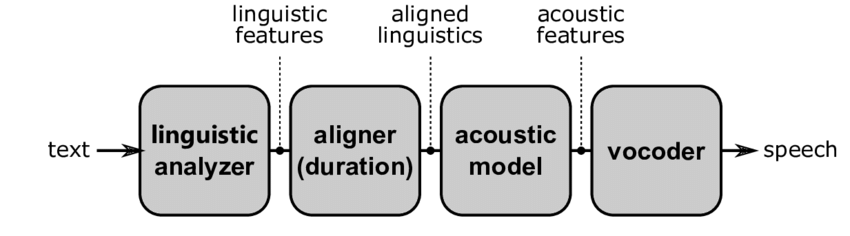
\includegraphics[width=0.7\textwidth,height=0.45\textheight,keepaspectratio]{images/audio-nlp/tts_pipeline.png}
    \end{center}
\end{frame}

\begin{frame}{Challenges in TTS}
\begin{itemize}
    \item Modern TTS systems face several practical and ethical challenges:

    \item \textbf{Prosody \& Emotion:}
    Generating natural intonation, emphasis, and expressive speech remains difficult.

    \item \textbf{Cross-Speaker Synthesis:}
    Voice cloning or multi-speaker synthesis requires adapting models to new voices without losing quality.

    \item \textbf{Low-Resource Languages:}
    Limited data makes it challenging to build high-quality TTS systems for many languages.

    \item \textbf{Ethical Issues:}
    Risk of misuse in deepfakes or generating fake celebrity voices.
\end{itemize}
\end{frame}
